\documentclass{beamer}

\mode<presentation> {

\usetheme{Madrid}

}
\usepackage{graphicx} % Allows including images
\usepackage{booktabs} % Allows the use of \toprule, \midrule and \bottomrule in tables
\usepackage{amsmath}
\usepackage[utf8]{inputenc} 
\usepackage[T1]{fontenc} 
\usepackage{lmodern} 
\usepackage{ngerman}
\usepackage{amsmath}
\usepackage{eurosym}
\usepackage{glossaries-extra}

%----------------------------------------------------------------------------------------
%	TITLE PAGE
%----------------------------------------------------------------------------------------

\title[Copulas]{Validität und Trennschärfe statistischer Tests in Abhängigkeit der Effektstärke einer Störvariable: Grundlagen} % The short title appears at the bottom of every slide, the full title is only on the title page

\author{Jonas Cedro Delgado} % Your name
\institute[Georg-August-Universität Göttingen] % Your institution as it will appear on the bottom of every slide, may be shorthand to save space
{
Georg-August-Universität Göttingen \\ % Your institution for the title page
\medskip

}
\date{\today} % Date, can be changed to a custom date

\begin{document}

\begin{frame}
\titlepage % Print the title page as the first slide
\end{frame}

\begin{frame}
\frametitle{Überblick} % Table of contents slide, comment this block out to remove it
\tableofcontents % Throughout your presentation, if you choose to use \section{} and \subsection{} commands, these will automatically be printed on this slide as an overview of your presentation
\end{frame}



%------------------------------------------------
\section{Grundbegriffe}
%------------------------------------------------
\frame{\sectionpage}


\begin{frame}
\frametitle{Validität vs. Trennschärfe eines Tests}

\end{frame}

\begin{frame}
\frametitle{Störfaktoren}
\begin{exampleblock}{Störfaktor:}
Ein Störfaktor (z. B. Bodenart) ist ein Faktor, welcher sowohl die abhängige Variable (z. B. Dünger) als auch die unabhängige Variable (z. B. Ertrag) beeinflussen könnte und nicht manipuliert werden kann. Störfaktoren können Merkmale von Untersuchungseinheiten oder äußere Faktoren sein. Störfaktoren sind als alternative oder konkurrierende Erklärungen zur Ausgangshypothese des Forschungsproblems zu sehen. Zur Kontrolle von Störfaktoren kann paarweise Zuordnung (Matching), oder Randomisierung angewandt werden.
\end{exampleblock}
\end{frame}

\begin{frame}
\frametitle{Blockbildung}
\begin{itemize}
\item Sind die Versuchseinheiten sehr unterschiedlich, dann wird die Isolierung interessierender Effekte (z. B. Ertrag einer Nutzpflanze) durch die Heterogenität des Materials (z. B. Bodenart) erschwert
\item Es empfiehlt sich Untergruppen von Untersuchungseinheiten zu bilden, die in sich gleichförmiger sind als das gesamte Material $\Rightarrow$ sog. \textit{homogene Versuchsblöcke}
\end{itemize}
\begin{exampleblock}{Blockbildung:}
Die Bildung von Blöcken homogener Untersuchungseinheiten wird \textit{Blockbildung} (Blocking) genannt. Innerhalb eines Blockes sind die Bedingungen homogener als Außerhalb und der Versuchsfehler wird i. A. kleiner. Durch Blocking können andere Effekte innerhalb der Blöcke verglichen werden; der Blockeffekt kann von anderen Effekten isoliert werden. Blöcke können zum Beispiel nebeneinanderliegenden Parzellen eines Feldes in einem landwirtschaftlichen Feldversuch sein.
\end{exampleblock}
\end{frame}

\begin{frame}
\frametitle{Randomisierung}
\begin{exampleblock}{Randomisierung (Zufallszuteilung):}
Unter Verwendung eines Zufallsmechanismus werden Untersuchungseinheiten unterschiedlichen Gruppen zugeordnet. Ziel ist das gleichmäßige verteilen bekannter und unbekannter an die Untersuchungseinheiten gebundene Störfaktoren auf Experimental- und Kontrollgruppe. Die Randomisierung soll die Zufälligkeit der Stichprobe im Sinne der mathematischen Statistik garantieren, entsprechend der Auswahl einer Zufallsstichprobe.
\end{exampleblock}
\end{frame}

\begin{frame}
\frametitle{Prinzipien der Versuchsplanung: Blockbildung und Randomisierung}
Die Blockbildung und die Randomisierung sind zwei der drei Prinzipien der Versuchsplanung.\footnote{Das Dritte Prinzip, die Wiederholung ist hier nicht relevant}. Beide dienen dazu, für alle anderen Einflussgrößen zu kontrollieren, sie also konstant zu halten.
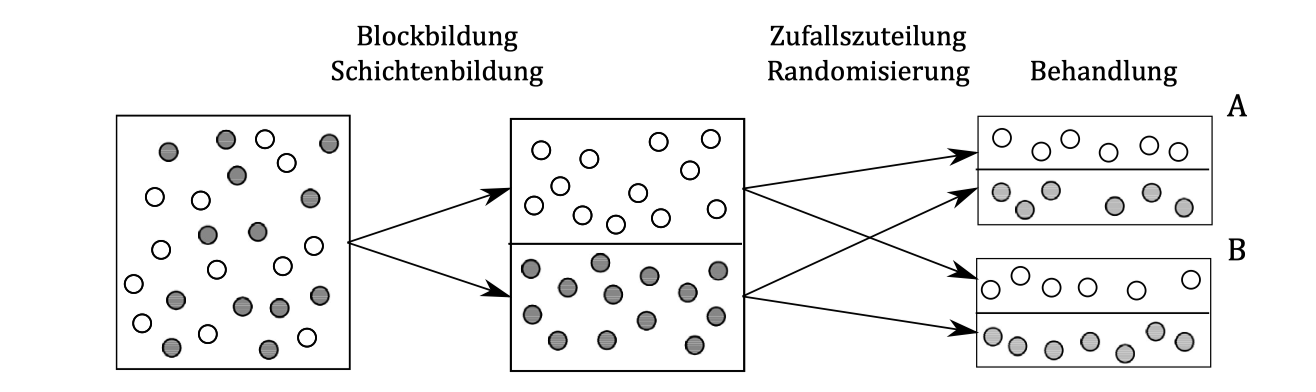
\includegraphics[scale=0.4]{/Users/jonascedrodelgado/Desktop/Practical/Praktikum/Template/Vortrag1/Blockbildung.png}
\caption{figure}{Diese Abbildung zeigt die Versuchsplanung für den Vergleich zweier Behandlungen: Sich unterscheidende Untersuchungseinheiten werden durch lokale Kontrolle (Blockbildung) getrennt erfasst und nach Zufallszuteilung (Randomisierung) zwei zu vergleichenden Einflüssen, Behandlungen (A und B), ausgesetzt. Quelle: Lothar Sachs, Jürgen Hedderich (2018).}
\end{frame}

\begin{frame}
\frametitle{Paarweise verbundener Versuchsplan}

\begin{exampleblock}{Paarweise verbundener Versuchsplan:}
Ein \textit{paarweise verbundener Versuchsplan} (paarweise verbundenes Design) ist ein Spezialfall eines \textit{randomisierten Blockversuchsplans} (randomisiertes Blockdesign). Ein paarweise verbundener Versuchsplan kann verwendet werden, wenn das Experiment nur zwei Behandlungsbedingungen hat und die Untersuchungseinheiten basierend auf einer Blockbildungsvariable in Paare zusammengefasst werden können. Die Untersuchungseinheiten werden dann innerhalb jedes Paares unterschiedlichen Behandlungsarten zufallszugeteilt (sog. Randomisierung)
\end{exampleblock}
\end{frame}

\begin{frame}
\frametitle{Paarweise verbundener Versuchsplan: Beispiel}
\begin{exampleblock}{Beispiel:}
Bei einer medizinischen Studie mit 1000 Versuchsteilnehmern bekommen alle Versuchsteilnehmer eine von zwei möglichen Behandlungsarten (Placebo oder Impfstoff). Die 1000 Teilnehmer sind in 500 verbundene Paare gruppiert. Jedes Paar ist auf Geschlecht und Alter abgestimmt. Zum Beispiel könnte Paar 1 zwei Frauen im Alter von 21 Jahren sein. Paar 2 könnte zwei Männer im Alter von 21 Jahren sein. Paar 3 könnte zwei Frauen im Alter von 22 Jahren sein und so weiter. Der paarweise verbundene Versuchsplan verwendet Randomisierung um für Störfaktoren zu kontrollieren. Hier kontrolliert der paarweise verbundene Versuchsplan für die zwei potenziellen Störfaktoren Alter und Geschlecht. Da der Versuchsplan paarweise verbunden ist kann er mittels eines gepaarten \textit{t}-Tests ausgewertet werden.
\end{exampleblock}
\end{frame}

\begin{frame}
\frametitle{Verbundene Stichproben}
Im verbundenen Zweistichprobenproblem werden bei jeder Untersuchungseinheit beide Verfahren betrachtet. Die Daten fallen also paarweise an. Es sei $x_{i}$ der Wert, der bei der $i$-ten Untersuchungseinheit beim ersten Verfahren beobachtet wird (z. B. Gabe eines spezifischen Düngers) und $y_{i}$ der Wert, der bei der $i$-ten Untersuchungseinheit beim zweiten Verfahren beobachten wird. Bei der $i$-ten Untersuchungseinheit wird also das Paar $(x_{i},y_{i})$ beobachtet (Realisierung der zweidimensionale Zufallsvariablen $(X_{i},Y_{i})$. Es soll überprüft werden, ob sich die beiden Verfahren unterscheiden. Besteht kein Unterschied zwischen den beiden Verfahren, sollte

 \[\operatorname{E}(X_{i}) = \operatorname{E}(Y_{i})\] bzw.  \[\operatorname{E}(D_{i}) =  \operatorname{E}(X_{i} - Y_{i}) = \operatorname{E}(X_{i}) -\operatorname{E}(Y_{i}) = 0\,.\] (Die Verteilung der Differenzen $D_{i}$ sollte das Zentrum null besitzen)
 
gelten

\end{frame}

\section{Gepaarter \textit{t}-Test}
\frame{\sectionpage}
\begin{frame}
\frametitle{Gepaarter \textit{t}-Test (verbundene Stichproben)}
Der gepaarte \textit{t}-Test testet im Falle, dass die Beobachtungen paarweise verbunden vorliegen, ob die Differenz von zwei Mittelwerten der Grundgesamtheit \[\mu_{D} = \mu_{X} - \mu_{Y}\] verschieden von einem spezifischen Wert $d_{0}$ ist.
\end{frame}

   
\begin{frame}
\frametitle{Gepaarter \textit{t}-Test (verbundene Stichproben)}

Seien $x_1, x_2, \dots, x_n$ und $y_1, y_2, \dots, y_n$ zwei verbundene Stichproben, die Realisierungen von $X_1, X_2, \dots, X_n  \; \stackrel{\mathrm{u.i.v.}}{\sim} \; \mathcal{N}(\mu_{x}, \sigma_{x}^2)$ und $Y_1, Y_2, \dots, Y_n  \; \stackrel{\mathrm{u.i.v.}}{\sim} \; \mathcal{N}(\mu_{y}, \sigma_{y}^2)$ darstellen. Es sei weiterhin angenommen, dass die Daten auf einer Intervall- oder Verhältnisskala gemessen wurden. Definiere $D_{i} = Y_{i} - X_{i}, \, i = 1, \ldots, n$. Sind $(X_i, Y_i)$ zweidimensional normalverteilt, dann gilt $D_{i} \sim \mathcal{N}(\mu_{d}, \sigma^2_{d})$, wobei $\mu_{d} = \mu_{y} - \mu_{x}$ und $\sigma_{d}^2 = \sigma_{x}^2 + \sigma_{y}^2 -2\sigma_{xy}$, mit $\sigma_{xy}  = \operatorname{Cov}(X_{i}, Y_{i})$. Die wahre Varianz $\sigma_{d}^2$ der Differenz wird durch die Stichprobenvarianz der Differenzen $S^2_{D}$ geschätzt.
\end{frame}

\begin{frame}
\frametitle{Testatistik (verbundene Stichproben)}

Für die Konstruktion der Teststatistik nutzt man aus, dass sich eine \textit{t}-verteilte Zufallsvariable aus der Division einer standardnormalverteilten Zufallsvariable durch die Quadratwurzel einer (um die Anzahl ihrer Freiheitsgrade korrigierten) Chi-Quadrat-verteilten Zufallsvariablen ergibt, d. h. 

\[t_n\equiv\frac{\mathcal{N}(0,1)}{\sqrt{\chi_n^2/n}}\,.\]

Die Testatistik für den gepaarten \textit{t}-Test ist gegeben durch:
\[ T=\sqrt{n}\frac{\overline{D}-d_0}{S_D}  \; \stackrel{H_0}{\sim} \; t_{n-1}\,,\]

wobei die Stichprobenstandardabweichung und das Stichprobenmittel gegeben sind durch $S_D = \sqrt{ \frac{1}{n-1}\sum_{i=1}^n (D_i-\overline{D})^2 }$ und $\overline{D} = \frac{1}n\sum_{i=1}^n D_i$

\end{frame}

\begin{frame}
\frametitle{Hypothesenspezifikation (verbundene Stichproben)}

Es ist möglich einen zweiseitigen, rechtsseitigen und linksseitigen Hypothesentest zu spezifizieren:
\begin{itemize}
\item $H_0\colon \mu_{d} = d_{0} \quad \text{vs.} \quad H_1\colon \mu_{d} \ne d_{0}$
\item $H_0\colon \mu_{d} \leq d_{0} \quad \text{vs.} \quad H_1\colon \mu_{d} > d_{0}$
\item $H_0\colon \mu_{d} \geq d_{0} \quad \text{vs.} \quad H_1\colon \mu_{d} < d_{0}$
\end{itemize}

mit den dazugehörigen Ablehnkriterien und Ablehnbereichen $A$:
\begin{itemize}
\item $|T|>t_{n-1, \alpha/2}$ und $A =(-\infty,-t_{1-\frac{\alpha}2;n-1}]\cup [t_{1-\frac{\alpha}2;n-1},\infty)$
\item $T>t_{n-1, 1-\alpha}$ und $A = [t_{1-\alpha;n-1},\infty)$
\item $T < t_{n-1, \alpha}$ und $A = (-\infty,-t_{1-\alpha;n-1}]$
\end{itemize}


\end{frame}

\begin{frame}
\frametitle{Vor- und Nachteile eines gepaarten \textit{t}-Tests}
\begin{itemize}
\item bietet den Vorteil, dass das Ergebnis des \textit{t}-Test valide ist (d. h. sein Ergebnis ist realitätsnah bzw. der Einfluss des Störfaktors wird "`herausgerechnet"')
\item Nachteil ist der Verlust an Freiheitsgraden. Da die Anzahl der Freiheitsgrade aufgrund der paarweisen Zuordnung geringer ist kann die Trennschärfe (Power) des Tests sinken (echte Unterschiede der Mittelwerte werden mit einer geringeren Wahrscheinlichkeit gefunden)
%\item $\Rightarrow$ {\color{red}{Es besteht eine Austauschbeziehung zwischen Validität und Trennschärfe}}
\item Eine Möglichkeit, um die Trennschärfe des Tests zu erhöhen besteht in einem vollen Ausschöpfen der Freiheitsgrade, da mit steigender Anzahl der Freiheitsgrade die Trennschärfe des Tests erhöht wird
\item Ein Test der die Freiheitsgrade voll ausschöpft (aber bzgl. der Validität als schlechter zu bewerten ist) ist der Zweistichproben-\textit{t}-Test für unverbundene Stichproben
\end{itemize}


\end{frame}

\section{Zweistichproben-\textit{t}-Test}
\frame{\sectionpage}
\begin{frame}
\frametitle{Zweistichproben-\textit{t}-Test (unverbundene Stichproben)}
Seien $X_1, X_2, \dots, X_n  \; \stackrel{\mathrm{u.i.v.}}{\sim} \; \mathcal{N}(\mu_{x}, \sigma_{x}^2)$ und $Y_1, Y_2, \dots, Y_m  \; \stackrel{\mathrm{u.i.v.}}{\sim} \; \mathcal{N}(\mu_{y}, \sigma_{y}^2)$ zwei unabhängige Zufallsstichproben. Es sei zunächst angenommen, dass $\sigma_{x} = \sigma_{y} = \sigma^2$. Dann gilt $X_{i} -Y_{i}  \; \stackrel{H_0}{\sim} \; \mathcal{N}(\mu_{x} -\mu{y}, 2\sigma^2)$ Da $\overline{X}\; \sim \;\mathcal{N}(\mu_{x}, \sigma^2/n) $ und $\overline{Y}\; \sim \;\mathcal{N}(\mu_{y}, \sigma^2/m) $ geeignete Schätzer für $\mu_{x}$ und $\mu_{y}$ sind und da $\overline{X} -\overline{Y}\; \sim \;\mathcal{N}(\mu_{x}-\mu{y},\sigma^2/n + \sigma^2/m) $ ist die Teststatistik gegeben durch:

\[T=\frac{\overline{X}-\overline{Y} - (\mu_{x}-\mu_{y})}{S_{p}\sqrt{\frac{1}{n}+\frac{1}{m}}}  \; \stackrel{H_0}{\sim} \; t_{n+m-2}\]

Hierbei wird die Größe

\[S_{p}^2=\frac{1}{n+m-2}\left(\sum_{i=1}^n (X_i-\overline X )^2 + \sum_{i=1}^n (Y_i-\overline Y )^2  \right)\]

als \textit{gepoolte Stichprobenvarianz} bezeichnet, da sie die Varianzen aus verschiedenen Stichproben kombiniert, indem sie ihr gewichtetes Mittel  verwendet, um die Gesamtvarianz zu erhalten.
\end{frame}
\begin{frame}
\frametitle{Hypothesenspezifikation (unverbundene Stichproben)}

Es ist möglich einen zweiseitigen, rechtsseitigen und linksseitigen Hypothesentest zu spezifizieren:
\begin{itemize}
\item $H_0\colon \mu_{x} = \mu_{y} \quad \text{vs.} \quad H_1\colon \mu_{x} \ne \mu_{y}$
\item $H_0\colon \mu_{x} \leq \mu_{y} \quad \text{vs.} \quad H_1\colon \mu_{x} > \mu_{y}$
\item $H_0\colon \mu_{x} \geq \mu_{y} \quad \text{vs.} \quad H_1\colon \mu_{x} < \mu_{y}$
\end{itemize}
mit den dazugehörigen Ablehnkriterien und Ablehnbereichen $A$:
\begin{itemize}
\item $|T|>t_{n+m-2, \alpha/2}$ und $A =(-\infty,-t_{1-\frac{\alpha}2;n+m-2}]\cup [t_{1-\frac{\alpha}2;n+m-2},\infty)$
\item $T>t_{n+m-2, 1-\alpha}$ und $A = [t_{1-\alpha;n+m-2},\infty)$
\item $T < t_{n+m-2, \alpha}$ und $A = (-\infty,-t_{1-\alpha;n+m-2}]$
\end{itemize}
Die Testentscheidung ergibt sich wie gewohnt aus dem Vergleich mit dem kritischen Wert.
\end{frame}

\section{Literatur}
\frame{\sectionpage}
\begin{frame}
\frametitle{Literatur}
 \begin{itemize}
\item[$\bullet$] Taeger, Dirk, und Sonja Kuhnt: \textit{Statistical hypothesis testing with SAS and R.} Chichester, UK, Wiley, 2014. pp. 23\\
\item[$\bullet$] Lothar Sachs, Jürgen Hedderich: \textit{Angewandte Statistik: Methodensammlung mit R.} 8., überarb. und erg. Auflage. Springer Spektrum, Berlin/ Heidelberg 2018.\\
\item[$\bullet$] Joseph Adler: \textit{R in a nutshell: A desktop quick reference.}, O'Reilly Media, Inc., 2010.\\
\item[$\bullet$] Handl, Andreas und Torben Kuhlenkasper: \textit{Einführung in die Statistik: Theorie und Praxis mit R.} Springer-Verlag, 2018.


\end{itemize}

\end{frame}


%------------------------------------------------



%------------------------------------------------




\end{document}